\begin{center}
  \section{\capitalisewords{Beyond RSA/ECDSA: the future of post-quantum cryptography}}
  Sreejit Roy Chowdhury, 1$^{st}$ Year, ECE
\end{center}

\setcounter{figure}{0}

\begin{multicols}{2}
  \begin{abstract}
    \bfseries
    The rapid advancement of quantum computing poses a significant threat to classical cryptographic
    systems such as RSA and Elliptic Curve Digital Signature Algorithm (ECDSA), which form the foundation of
    modern digital security. Quantum algorithms, particularly Shor’s algorithm, have the potential to efficiently
    solve the mathematical problems underlying these cryptographic techniques, thereby compromising the
    confidentiality, integrity, and authenticity of digital communications. Post-Quantum Cryptography (PQC) has
    emerged as a promising solution to address these challenges by developing cryptographic algorithms that are
    resistant to attacks from both classical and quantum computers.

    \noindent
    This paper presents an overview of post-quantum cryptography, its importance in the era of quantum computing,
    and the major categories of quantum-resistant algorithms, including lattice-based, hash-based, code-based, and
    multivariate cryptographic systems. The study also highlights the standardization efforts led by the National
    Institute of Standards and Technology (NIST) and discusses widely recognized algorithms such as CRYSTALS-
    Kyber and CRYSTALS-Dilithium. Furthermore, the paper examines the practical challenges associated with the
    implementation and migration of PQC in real-world systems. The objective of this work is to provide a
    comprehensive understanding of the need for quantum-safe security mechanisms and the future direction of
    cryptographic research in the post-quantum era.

    \vspace{1em}
    {\justifying\noindent\textbf{Keywords:} Post-Quantum Cryptography, Quantum Computing, RSA, ECDSA, Shor’s Algorithm,
    Quantum-Resistant Security, Cryptography, NIST, CRYSTALS-Kyber, CRYSTALS-Dilithium.\par}
  \end{abstract}

  \subsection*{\centering\uppercase{INTRODUCTION}}
  In today’s digital world, cryptography plays a major role in protecting communication, online transactions,
  banking systems, passwords, and cryptocurrencies such as Bitcoin. Every time a user sends a message, logs into
  a website, or makes an online payment, cryptographic algorithms work in the background to keep the
  information safe from attackers.Modern internet security mainly depends on classical cryptographic systems
  such as RSA and Elliptic Curve Digital Signature Algorithm (ECDSA). RSA is a public-key cryptographic
  algorithm that secures communication using very large prime numbers, while ECDSA uses mathematical
  properties of elliptic curves to create secure digital signatures. These algorithms are currently trusted because
  classical computers require an extremely long time to solve the mathematical problems behind them.

  \noindent
  For example, Bitcoin uses ECDSA to protect wallet ownership and digital signatures. A Bitcoin wallet address
  is linked to a private key, and only the owner of that private key can authorize transactions. Bitcoin also uses the
  SHA-256 hashing algorithm to secure blocks and maintain the integrity of the blockchain. At present, breaking
  these systems using ordinary computers is practically impossible due to the astronomically large search space of
  \(2048^{12}\) combinations of seed phrases. However, the development of quantum computers has created new
  concerns in the field of cybersecurity. Unlike classical computers that process information using bits (0 or 1),
  quantum computers use qubits, which can exist in multiple states simultaneously. In the future, large-scale
  quantum computers with stable logical qubits may become powerful enough to solve certain mathematical
  problems much faster than classical computers. Thus, the need to bring Quantum-resistant security measures
  increases each passing day.

  \subsection*{\centering\uppercase{Public-Key Cryptography: RSA and ECDSA Foundations}}
  RSA and ECDSA are widely used public-key cryptographic systems that secure modern digital
  communication, online banking, secure web services, and cryptocurrencies such as Bitcoin. Their
  security is based on mathematical problems that are computationally difficult for classical computers.

  \noindent
  RSA is based on number theory and relies on the difficulty of factoring a large composite number into
  its prime factors. A public key is used for encryption, while a mathematically related private key is
  used for decryption. Although key generation is straightforward, breaking the system without the
  private key is infeasible because factoring large integers becomes extremely time-consuming as key
  sizes increase.

  \begin{center}
\vspace{-0.5em}
\begin{minipage}{0.98\columnwidth}
\centering
    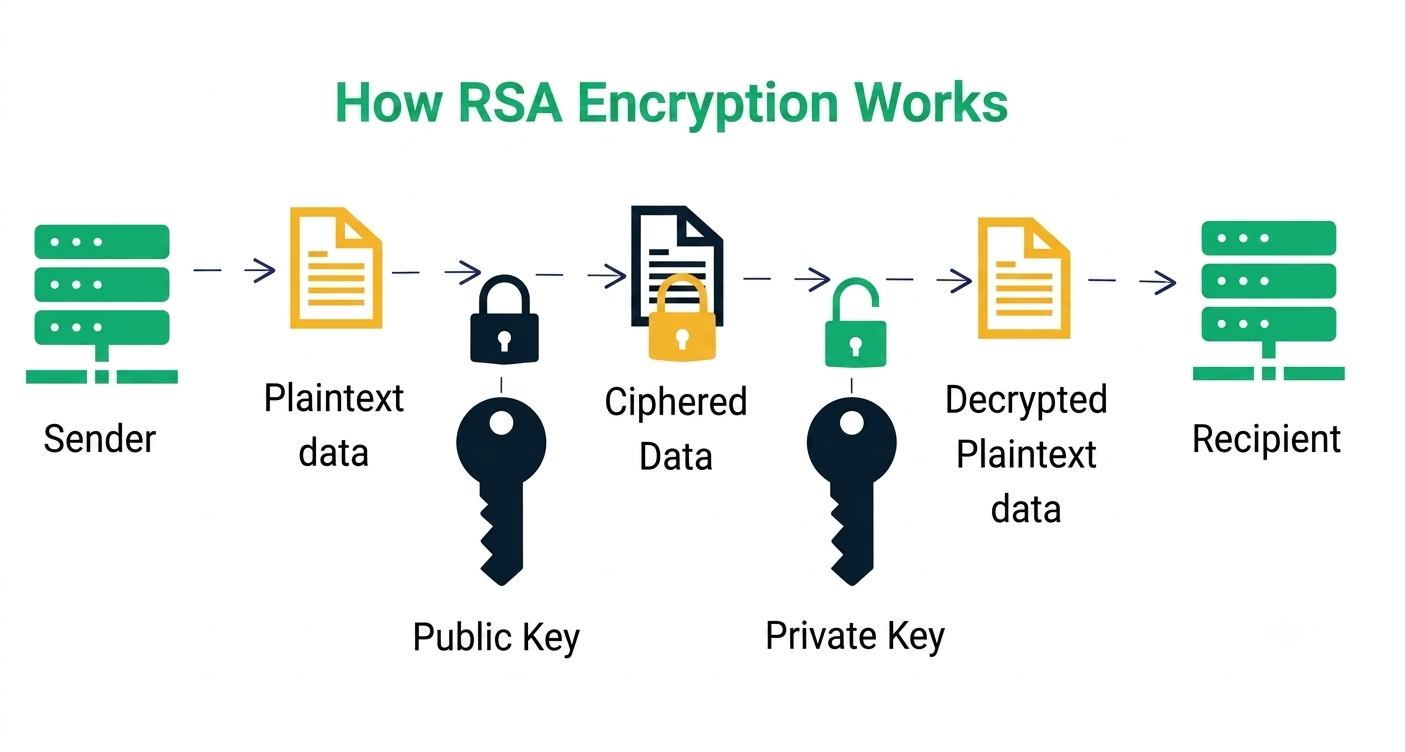
\includegraphics[width=0.9\columnwidth]{assets/images/RSA.png}
    \captionof{figure}{RSA}
\end{minipage}
  \end{center}

  ECDSA is based on elliptic curve cryptography over finite fields. A private key is a randomly selected
  number, and the corresponding public key is generated using elliptic curve point multiplication with a
  fixed generator point (G). Digital signatures are created using cryptographic hashing combined with
  elliptic curve operations, and verification is possible without revealing the private key. The security of
  ECDSA depends on the elliptic curve discrete logarithm problem, which makes it computationally
  infeasible to derive the private key from the public key using classical computing methods.

  \noindent
  Both RSA and ECDSA are widely deployed in real-world systems, including HTTPS/TLS protocols,
  secure messaging, and blockchain-based cryptocurrencies like Bitcoin.

  \noindent
  However, their security is based on mathematical hardness assumptions rather than absolute
  guarantees. This means that future advancements in quantum computing could potentially weaken
  these systems by solving their underlying mathematical problems more efficiently, motivating the
  development of post-quantum cryptography.

  \begin{center}
\vspace{-0.5em}
\begin{minipage}{0.98\columnwidth}
\centering
    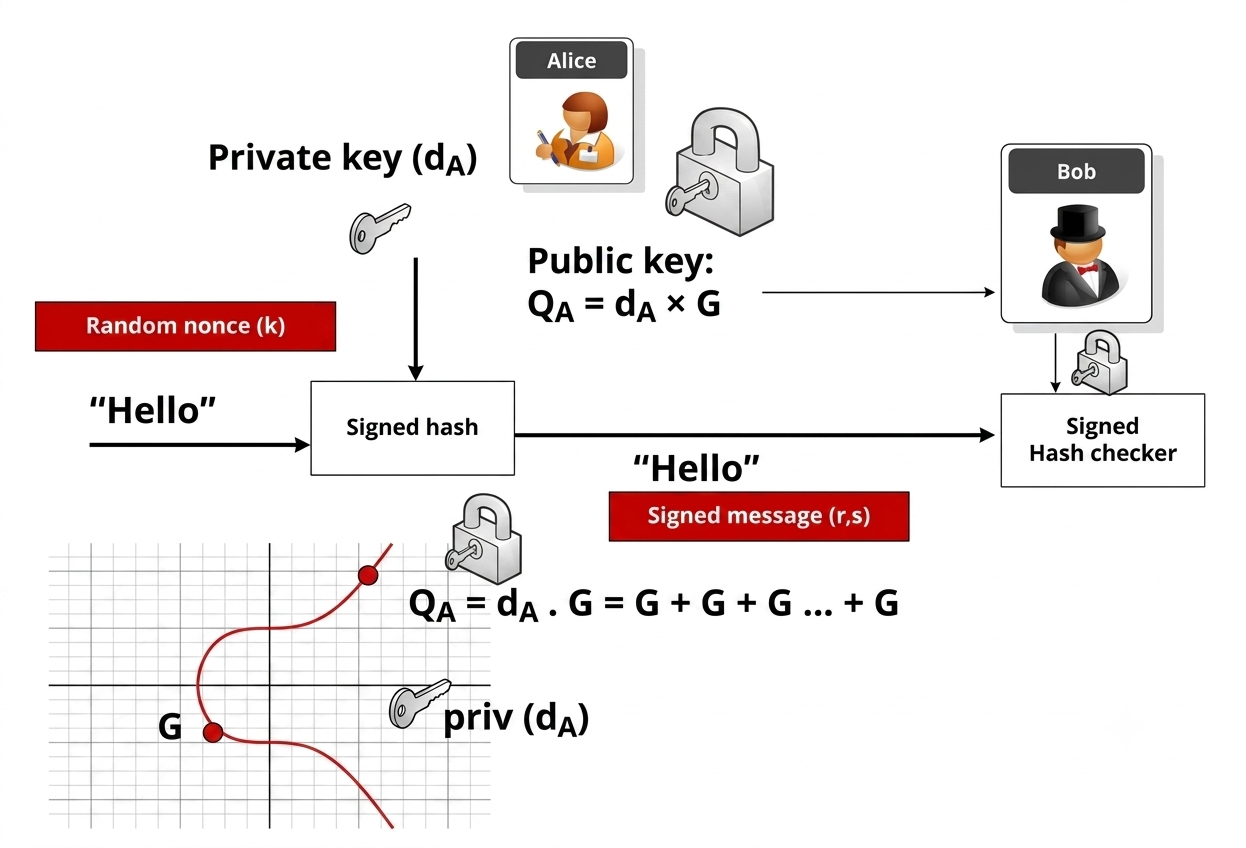
\includegraphics[width=0.9\columnwidth]{assets/images/ECDSA.png}
    \captionof{figure}{ECDSA}
\end{minipage}
  \end{center}

  With ECDSA, Alice will sign a message with her private key (d), and then Bob will use her public
  key to verify that she signed the message (and that the message has now changed):

  \noindent
  Alice signs the message with the following:
  \begin{enumerate}
    \item Create a hash of the message \(e=\operatorname{HASH}(m)\).
    \item Let \(h\) be the \(L_n\) be the leftmost bits of \(e\), \(L_n\) has a bit length of the group order \(N\).
    \item Create a random number \(k\) which is between \(1\) and \(N-1\).
    \item Calculate a point on the curve as \((x_1,y_1)=k\times G\).
    \item Calculate \(r=x_1\pmod N\). If \(r=0\), go back to Step 3.
    \item Calculate \(s=k^{-1}(h+r d_A)\pmod N\). If \(s=0\), go back to Step 3.
    \item The signature is the pair \((r,s)\).
  \end{enumerate}

  Bob will check with:
  \begin{enumerate}
    \item Create a hash of the message \(e=\operatorname{HASH}(m)\).
    \item Let \(h\) be the \(L_n\) leftmost bits of \(e\).
    \item Calculate \(c=s^{-1}\pmod N\).
    \item Calculate \(u_1=h\cdot c\pmod N\) and \(u_2=r\cdot c\pmod N\).
    \item Calculate the curve point \((x_1,y_1)=u_1\times G+u_2\times Q_A\). If \((x_1,y_1)=\mathcal{O}\), then the signature is
      invalid.
  \end{enumerate}

  \begin{center}
\vspace{-0.5em}
\begin{minipage}{0.98\columnwidth}
\centering
    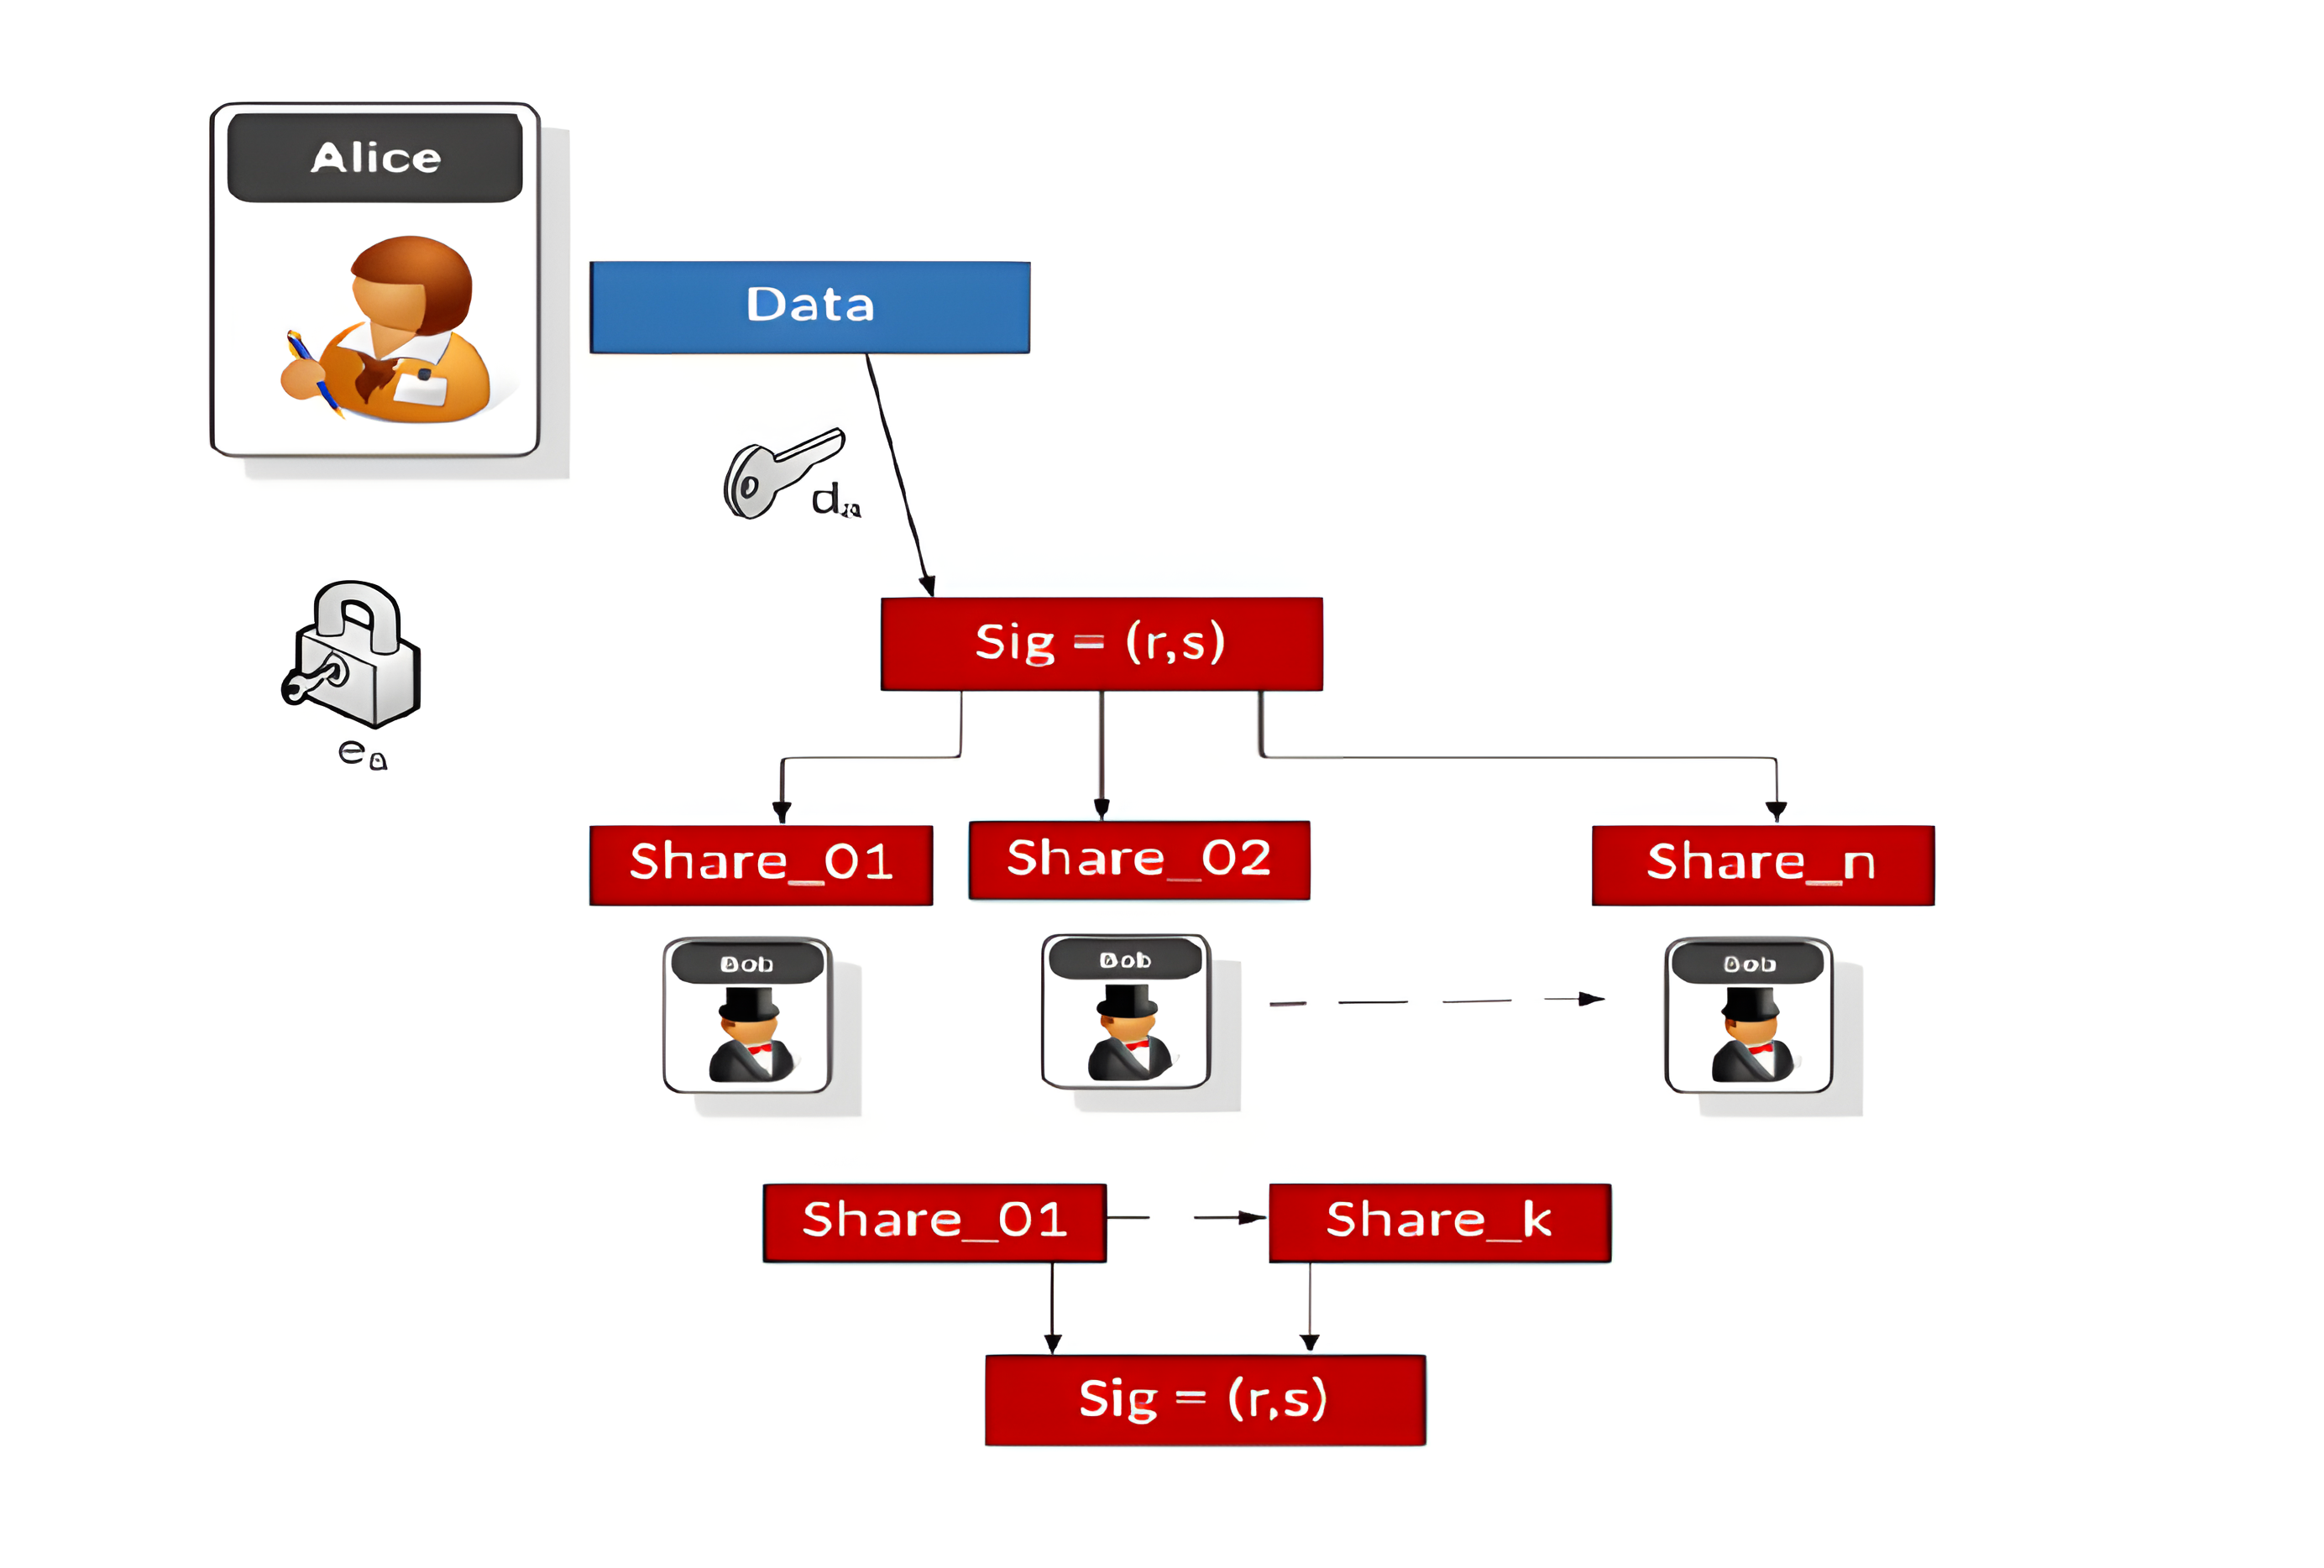
\includegraphics[width=0.9\columnwidth]{assets/images/ECDSA(1).png}
    \captionof{figure}{ECDSA}
\end{minipage}
  \end{center}
\vspace{-0.35em}

  \subsection*{\centering\uppercase{Quantum Threats to Classical Cryptography}}
  The primary motivation for post-quantum cryptography is the potential ability of quantum computers
  to break widely used cryptographic systems such as RSA and ECDSA. This threat is mainly based on
  Shor’s algorithm, which theoretically allows a sufficiently powerful quantum computer to solve
  integer factorization and discrete logarithm problems efficiently. Since RSA security depends on
  factoring large composite numbers and ECDSA depends on the elliptic curve discrete logarithm
  problem, both systems would become vulnerable if such quantum capability is achieved.

  \noindent
  In a real-world scenario, this means that a public key, which is openly shared during secure
  communication or stored on blockchain networks, could be used by an attacker to compute the
  corresponding private key. For example, in cryptocurrencies like Bitcoin, if a user’s public key is
  exposed, a powerful quantum computer could potentially derive the private key and authorize
  unauthorized transactions. Similarly, in internet security protocols such as HTTPS, intercepted
  communications that rely on classical public-key exchanges could be decrypted if private keys are
  recovered.

  \noindent
  Although current quantum computers are not capable of executing such attacks due to limitations in
  qubit stability and error correction, the theoretical risk remains significant. Google and the Dutch
  institute CWI officially broke the SHA-1 algorithm in 2017. They achieved this by producing a
  "collision"—where two entirely different files generate the same cryptographic fingerprint. It was
  broken using classical computing techniques not even quantum computers, this shows what powerful
  quantum computers can do to more powerful algorithms like HASH 160 and SHA256 which
  especially protects bitcoin wallets in future if not upgraded carefully. As a result SHA-1 is officially
  deprecated and is replaced by SHA-2 and SHA-3 for modern internet services.

  \noindent
  The transition to fault-tolerant quantum computers with a large number of logical qubits is still an
  open challenge, but once achieved, it could fundamentally change the security assumptions of modern
  cryptography.

  \subsection*{\centering\uppercase{Securing the Future: Quantum-Resistant Solutions}}
  To address the potential failure of RSA and ECDSA in a future where large-scale quantum computers
  exist, researchers have developed post-quantum cryptography (PQC), which focuses on cryptographic
  systems that remain secure even against quantum attacks. The key idea is to replace current schemes
  with alternatives that are not based on integer factorization or discrete logarithm problems, since these
  can be efficiently solved using Shor’s algorithm.

  \noindent
  One of the most promising approaches is lattice-based cryptography, which relies on hard problems in
  high-dimensional geometric structures called lattices. These problems, such as the Learning With
  Errors (LWE) problem, are believed to remain difficult even for quantum computers. Lattice-based
  schemes are currently considered the leading candidate for replacing both encryption and digital
  signature systems due to their balance of security and performance. Another important category is
  hash-based cryptography, which uses secure hash functions to build digital signatures that are highly
  resistant to quantum attacks, although they often come with larger signature sizes.

  \noindent
  Quantum cryptography emerging as another option, secures data transmission using the immutable
  laws of physics rather than complex mathematics that are currently in use in algorithms like
  RSA/ECDSA. Its primary application, \textbf{Quantum Key Distribution (QKD)}, utilizes particles of light
  (photons) to share encryption keys. Any attempt by an unauthorized third party to intercept or read
  the transmission alters the quantum state. This wave-function collapse instantly introduces
  detectable anomalies, exposing the eavesdropper governed by \textbf{Heisenberg Uncertainty Principle}.

  \noindent
  Code-based cryptography, such as systems derived from error-correcting codes, is another alternative
  that has shown strong resistance to both classical and quantum attacks, though it often suffers from
  large key sizes. These approaches are being actively evaluated and standardized by global research
  efforts, particularly those led by international security organizations.

  \begin{center}
\vspace{-0.5em}
\begin{minipage}{0.98\columnwidth}
\centering
    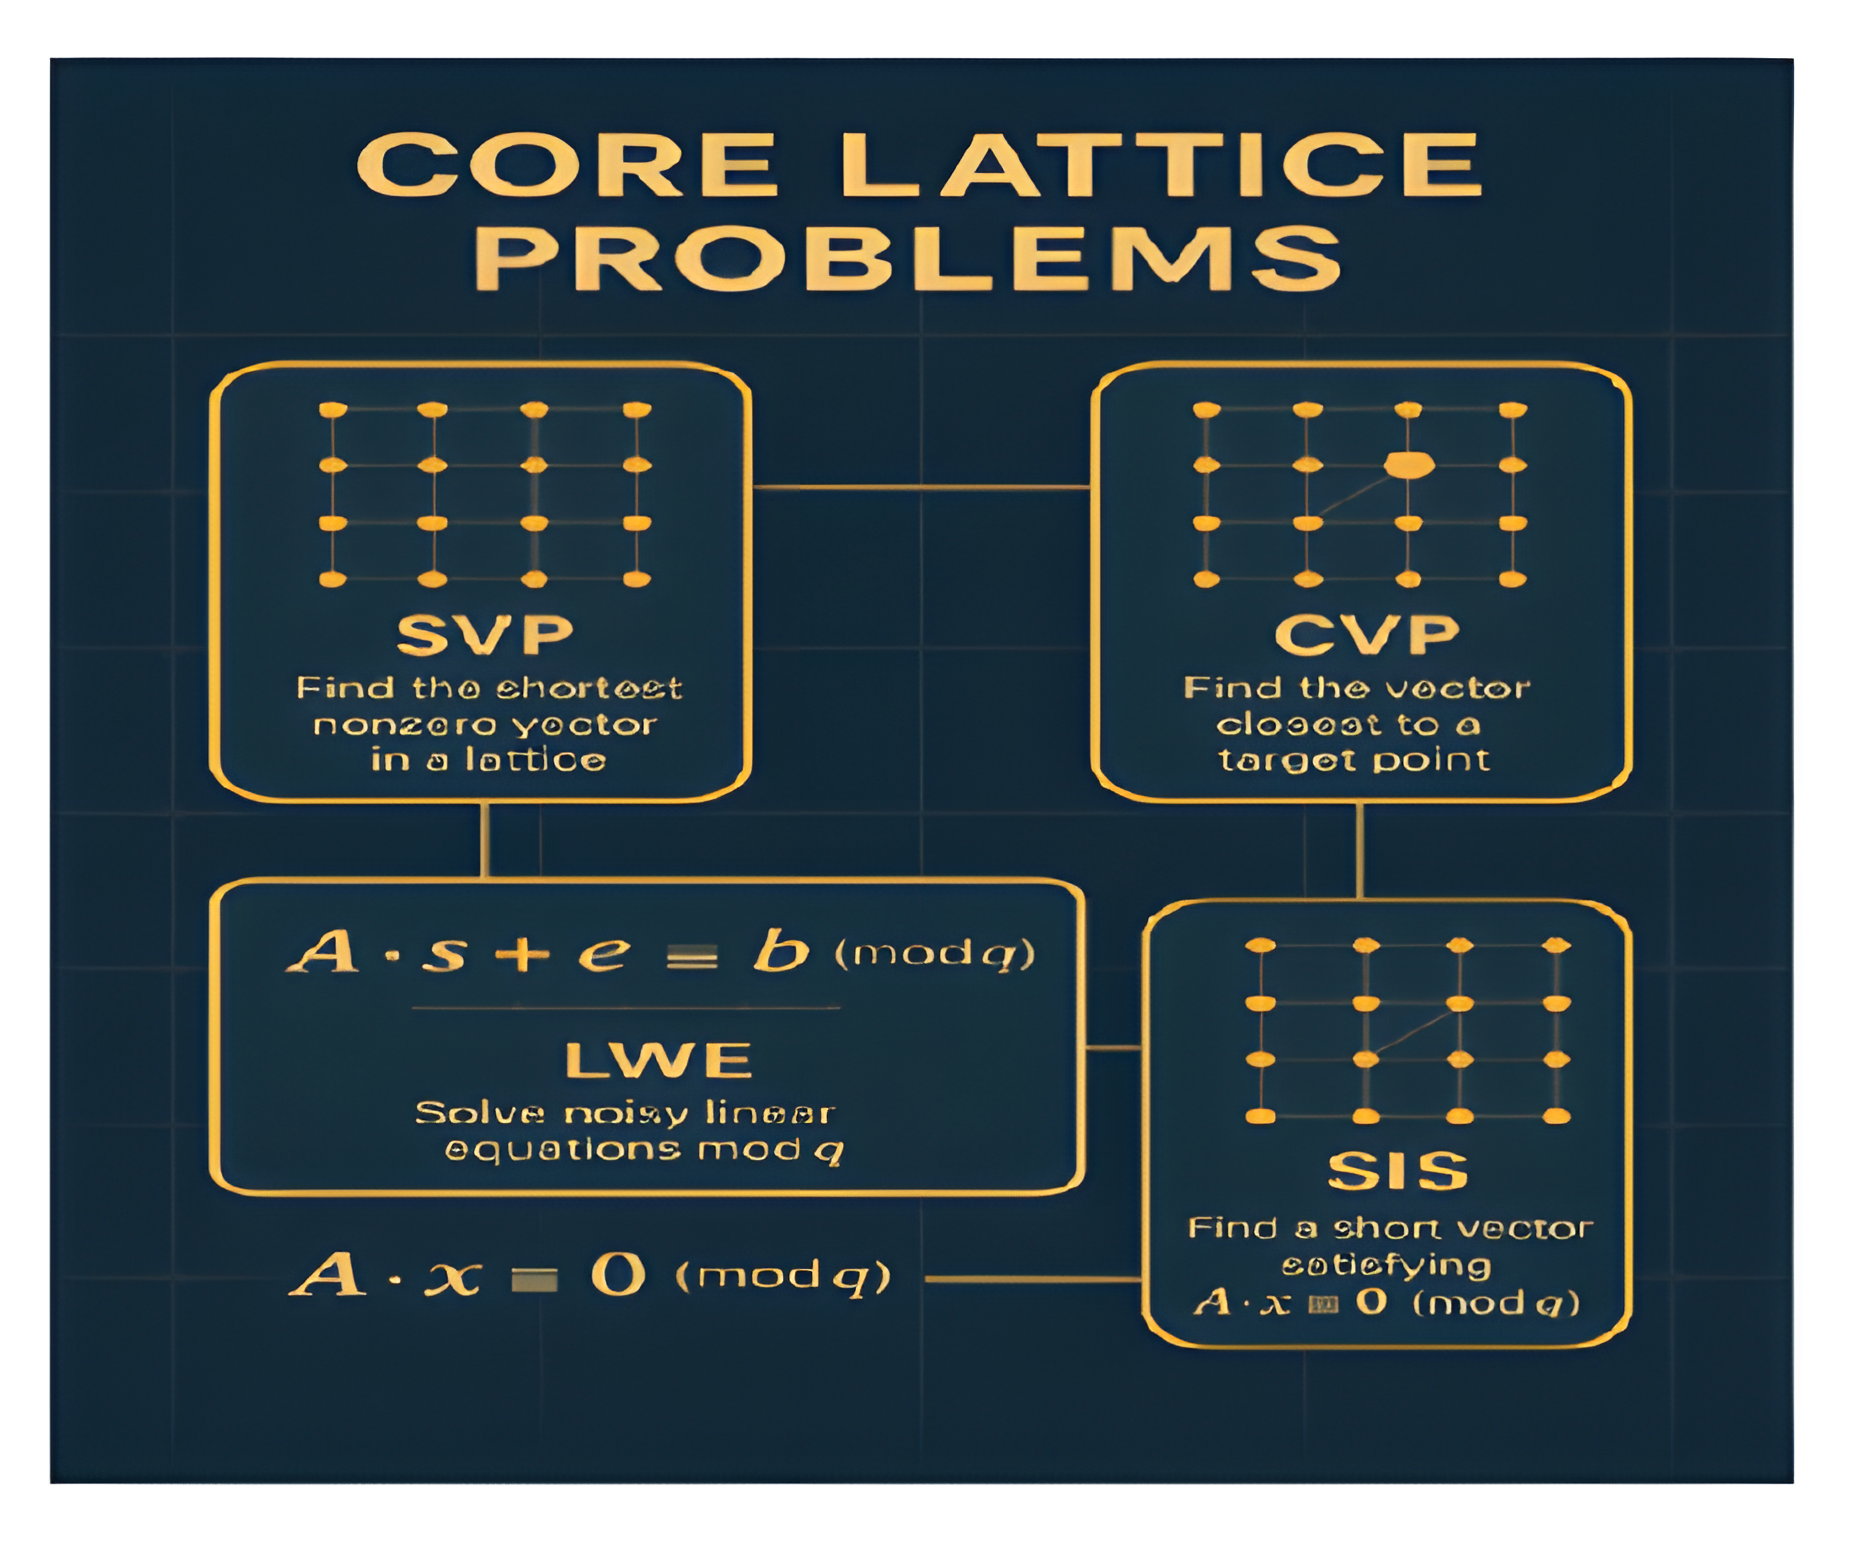
\includegraphics[width=0.6\columnwidth]{assets/images/CLP.png}
    \captionof{figure}{Core Lattice Problems}
\end{minipage}
  \end{center}
\vspace{-0.35em}

  \subsection*{\centering\uppercase{Standardization and Hybrid Cryptographic Transition}}
  To ensure a secure transition toward a quantum-safe future, global standardization efforts are being
  led by the National Institute of Standards and Technology (NIST), which has selected and
  recommended several post-quantum cryptographic algorithms for real-world deployment. Among
  these, CRYSTALS-Kyber has been chosen for key encapsulation mechanisms due to its strong
  security based on lattice problems and its relatively efficient performance compared to other
  candidates. Similarly, CRYSTALS-Dilithium has been selected for digital signatures, providing a
  practical replacement for RSA and ECDSA in many applications.

  \noindent
  In practice, the migration from classical to post-quantum cryptography is expected to follow a hybrid
  approach, where both traditional algorithms and post-quantum algorithms are used together. This
  hybrid cryptographic model ensures backward compatibility while gradually introducing quantum-
  resistant security. It allows systems to remain secure even if one of the underlying schemes is later
  found to be weaker than expected, thereby reducing migration risk.

  \noindent
  This transition phase is critical because global infrastructure, including secure communication
  protocols and blockchain systems, cannot be changed instantly. Therefore, hybrid cryptography
  provides a practical bridge between current security systems and fully post-quantum secure
  architectures.

  \subsection*{\centering\uppercase{Practical Constraints}}
  One of the practical responses to quantum-related security concerns is strengthening existing
  symmetric cryptographic and hashing systems rather than replacing them entirely. For example,
  algorithms such as SHA-256 can be upgraded to SHA-512 to increase the output size and
  computational resistance. While quantum algorithms like Grover’s algorithm can theoretically reduce
  the effective security strength of hash functions, increasing the hash size helps maintain a higher
  security margin even in a post-quantum environment. This approach is relatively simple because hash
  functions are not broken in the same fundamental way as RSA or ECDSA under quantum attacks.

  \noindent
  However, increasing security strength is not only about choosing larger algorithms, but also about
  balancing efficiency and system constraints. Larger hash outputs, such as those in SHA-512, increase
  computational overhead, storage requirements, and bandwidth usage, which may impact performance
  in large-scale systems like blockchain networks and distributed applications. This creates a trade-off
  between security level and practical efficiency.

  \noindent
  \textbf{The "Harvest Now, Decrypt Later" Threat:} Attackers are actively intercepting and storing
  encrypted data today to decrypt it later once quantum computers are viable. This pressures
  organizations to act now, even though PQC standards and browser trust store adoptions are still
  evolving.

  \noindent
  The main objective in post-quantum security design is therefore not only to maximize resistance
  against attacks, but to achieve strong security with minimal computational and storage cost. In other
  words, the goal is to improve security without significantly increasing sample size, key size, or system
  complexity. This balance is critical for real-world adoption, where millions of devices and systems
  must operate efficiently while still remaining secure against both classical and quantum threats.

  \subsection*{\centering\uppercase{Conclusion}}
  Post-quantum cryptography represents a necessary evolution of modern security systems in response
  to the theoretical capabilities of quantum computing. While RSA and ECDSA currently provide
  strong protection for digital communication, financial systems, and blockchain networks, their
  security is fundamentally based on mathematical assumptions that may not hold in a future quantum-
  enabled environment. The development of quantum algorithms such as Shor’s algorithm highlights
  that problems once considered computationally infeasible could become solvable, changing the
  foundation of trust in today’s digital infrastructure.

  \noindent
  In response to this potential risk, global efforts such as those led by NIST have introduced post-
  quantum standards, including CRYSTALS-Kyber for key encapsulation and CRYSTALS-Dilithium
  for digital signatures. Along with hybrid cryptographic approaches, these solutions aim to ensure a
  smooth transition from classical to quantum-resistant systems without disrupting existing
  infrastructure. However, the effectiveness of these solutions ultimately depends on how accurately
  future quantum capabilities are estimated and how quickly real-world systems can adapt.

  \noindent
  This leads to an important question: what if quantum computing reaches practical power sooner than
  expected? What if, one random day you open your eyes encrypted messages can be decrypted
  instantly, digital signatures can be forged, and cryptocurrency funds can disappear or be redirected
  without detection and authorization ? The uncertainty surrounding this possibility is precisely what
  makes post-quantum cryptography not just a theoretical study, but a critical requirement for the future
  of global digital security.

  \subsection*{\centering\uppercase{References}}
  \begin{justify}
  \Urlmuskip=0mu plus 1mu\relax
  \begin{enumerate}
    \item P. W. Shor, “Algorithms for quantum computation: Discrete logarithms and
      factoring,” Proceedings of the 35th Annual Symposium on Foundations of Computer
      Science, 1994.
    \item D. E. Shor, “Polynomial-time algorithms for prime factorization and discrete
      logarithms on a quantum computer,” SIAM Journal on Computing, vol. 26, no. 5,
      1997.
    \item National Institute of Standards and Technology (NIST), “Post-Quantum
      Cryptography Standardization Project,” 2024. \url{https://csrc.nist.gov/projects/post-quantum-cryptography}
      \item NIST, “FIPS 203: Module-Lattice-Based Key-Encapsulation Mechanism Standard
      (ML-KEM / CRYSTALS-Kyber),” 2024.
      \item \url{https://asecuritysite.com/ecdsa/ecdsa4}
      \item J. Buchmann, “Introduction to Cryptography,” Springer, 2017.
      \item D. J. Bernstein, “Post-quantum cryptography,” Communications of the ACM, vol. 61,
      no. 2, pp. 72--80, 2018.
  \end{enumerate}
  \end{justify}
\end{multicols}
% Full-width info box outside multicols
\begin{center}
  \begin{minipage}{\textwidth}
    \begin{tcolorbox}[
  colback=SoftYellow,
  colframe=IEEEblue!70!black,
  boxrule=0.5pt,
  arc=0mm,
  left=3mm, right=3mm, top=2.5mm, bottom=2.5mm
]
\small\RaggedRight \textbf{\color{IEEEblue!75!black}Did you know?} — \textbf{ECE Workbench:} \textbf{LTspice} simulates, \textbf{KiCad} draws PCB (run ERC/DRC), \textbf{PlatformIO} uploads, \textbf{MATLAB/Python} does FFT, \textbf{Git} tracks versions. \textit{Tip:} note units (\texttt{// 3.3V}) and commit often.
\end{tcolorbox}

  \end{minipage}
\end{center}